\documentclass{article}
\usepackage[utf8]{inputenc}
\usepackage{graphicx}
\usepackage{biblatex}
\usepackage{flafter}
\usepackage{float}
\usepackage{graphicx}
\usepackage{booktabs}
\usepackage{placeins}

\addbibresource{bibliography.bib}
\newcommand{\beginsupplement}{%
        \setcounter{table}{0}
        \renewcommand{\thetable}{S\arabic{table}}%
        \setcounter{figure}{0}
        \renewcommand{\thefigure}{S\arabic{figure}}%
     }
\title{The genetic background of Cambodian pneumococcal carriage isolates following PCV13}
\author{Sophie Belman, Stephanie Lo, Sona Soeng, 
\\Rebecca Gladstone, Keith Klugman, Robert Breiman, 
\\Lesley McGee, Stephen Bentley, Paul Turner}
\date{January 2021}

\begin{document}
\maketitle
\section{Abstract}
Background: We sought to elucidate the genetic background of the perturbation by PCV13 to the \textit{Streptococcus pneumoniae} strain and serotype composition in Cambodian carriage isolates.
\\Methods: Pre-PCV13 (01/2013–12/2015, N=258) and the post-PCV13 isolates (01/2016-02/2017, N=428) were sequenced and analysed using PopPUNK and SeroBA to determine strain prevalence and serotype composition. Antibiotic susceptibility was predicted using the CDC-antimicrobial resistance (AMR) pipeline and concordance with phenotypic data was determined.
\\Results: Following PCV13 implementation in Cambodia a significant expansion of non-vaccine type (NVT) serotypes 23A, 34, and 6D occurred on the genetic background of diverse strains comprising over three serotypes  (GPSC16) and non-diverse strains comprising a single serotype (GPSC626 and GPSC45). The bioinformatics pipeline developed by the CDC resulted in 90\% concordance with the phenotypic antimicrobial susceptibility testing. Expanding serotypes are significantly associated with AMR. There is a significant association between vaccine serotypes and antimicrobial resistance.
\\Conclusion: The strain population in Cambodia has been perturbed by PCV13 resulting in expansion of some NVT serotypes. Although there is an overall decrease in AMR in the population the strains comprising the expanding NVTs are associated with AMR. Further evaluation of successful strains may further elucidate any genetic drivers of proliferation following PCV13. Collection of additional carriage isolates is ongoing in this population.
\section{Introduction}
\textit{Streptococcus pneumoniae} (the pneumococcus) is an opportunistic pathogen whose colonization is a prerequisite for disease. Its occupation of the nasopharyngeal passage has a range of outcomes from asymptomatic carriage to life-threatening invasive pneumococcal disease (IPD)\cite{weiserStreptococcusPneumoniaeTransmission2018}. Estimates of pneumococcal related deaths in 2015 were around 500,000\cite{wahlBurdenStreptococcusPneumoniae2018}. There is known to be under detection in high-mortality developing countries due to limited access to healthcare and antibiotic use prior to testing making this a likely underestimate \cite{obrienBurdenDiseaseCaused2009,troegerEstimatesGlobalRegional2017}.
\\The globally implemented vaccine is a pneumococcal conjugate vaccine (PCV) targeting up to 13 capsular serotypes (1, 3, 4, 5, 6A, 6B, 7F, 9V, 14, 18C, 19A, 19F, 23F) that account for most of the disease in infants\cite{VaccineInformationStatement2019}. This vaccine was broadly used in 145 countries by 2020 and has substantially reduced vaccine serotype (VT) associated pneumococcal disease among children\cite{pilishviliSustainedReductionsInvasive2010,vongottbergEffectsVaccinationInvasive2014}. Furthermore, there was an estimated 51\% decline in pneumococcal related deaths globally from 2000 to 2015 and can likely be explained by global deployment of PCV\cite{wahlBurdenStreptococcusPneumoniae2018}.  
\\Currently over 100 capsular serotypes have been identified on genetic backbones of over 800 strains globally; called Global Pneumococcal Sequence Clusters (GPSCs). It is not uncommon for a single GPSC to undergo capsular switching and express different serotypes. Some GPSC’s have a propensity for high diversity of capsular types while others are restricted to a few\cite{loPneumococcalLineagesAssociated2019}. GPSCs represent the genetic backbone of the pneumococcus and will henceforth be referred to as GPSCs and strains interchangeably. The implementation of PCV clears the niche for expansion of non-vaccine types (NVT). Understanding the genetic background upon which vaccine-related serotype switching occurs can further elucidate strains with the potential to perpetuate troublesome phenotypes such as antibiotic resistance and association with IPD. Understanding the strains driving post-vaccine serotype expansion will be key for future vaccine design\cite{loPneumococcalLineagesAssociated2019}. 
\\PCVs are designed to remove target serotypes from carriage in the nasopharynx to protect children from pneumococcal infections. As the main reservoirs, children are the primary transmission vectors \cite{bogaertStreptococcusPneumoniaeColonisation2004,wyllieMolecularSurveillanceStreptococcus2016} for pneumococci. As such its population ecology within the nasopharynx of children is an indicator of IPD prevalence and vaccine impact within a population\cite{hamalubaCrossSectionalObservationalStudy2015}. 
\\In Cambodia, pneumococcal pneumonia was the leading cause of lower respiratory infection associated with death in children under 5 and the second leading cause of morbidity and mortality as measured in 2015 \cite{gbd2015mortalityandcausesofdeathcollaboratorsGlobalRegionalNational2016}. In the same year, PCV-13 was included in the national childhood vaccination schedule. Several studies elucidating serotype distribution have been conducted in Cambodia, however contextualizing these serotypes by their genetic background and continued evaluation of the population ecology is necessary to both determine vaccine impact and elucidate strains which are driving any post-PCV upswing in disease\cite{inghammarSerotypeDistributionClinical2018,turnerPneumococcalInfectionChildren2015,mooreCharacterisationInvasiveStreptococcus2016,turnerImpact13ValentPneumococcal2020}.Disease and carriage populations do not exist in isolation from one another – the prevalence in one likely reflects the eventual prevalence of the other. Understanding the genetic background of carriage populations regionally can indicate which serotypes may emerge following PCV13 and may elucidate future drivers of IPD. This study aims to characterize the impact of PCV-13 on the GPSC and serotype prevalence pre- and post-PCV13 implementation in a Cambodian carriage population. 
\section{Methods}
\subsection{Bacterial isolate collection}
These isolates were collected as part of a larger study conducted by Turner et.al 2015\cite{turnerPneumococcalInfectionChildren2015}. Nasopharyngeal \textit{S. pneumoniae} was isolated from healthy children under 5 years old upon admission to the Angkor Hospital, in Siem Reap, Cambodia between 2013 and 2017. 
\subsection{Microbiology and sequencing}
These samples were selectively cultured on BD™ Trypticase™ Soy Agar II with 5\% sheep blood (Beckton Dickinson, Heidelberg, Germany) and incubated overnight at 37 °C in 5\% CO2. Genomic DNA was then extracted manually using a modified QIAamp® DNA Mini Kit (QIAGEN, Inc., Valencia, CA) protocol. As part of the Global Pneumococcal Sequencing (GPS) Project, pneumococcal isolates were whole-genome sequenced on the Illumina HiSeq platform to produce paired-end reads with an average of 100-125 bases in length and data were deposited in the European Nucleotide Database. WGS data was processed as previously described\cite{gladstoneInternationalGenomicDefinition2019}. Phenotypic antimicrobial susceptibility testing was conducted against penicillin (PEN), erythromycin (ERY), cefotaxime (CTX), co-trimoxazole (COT), chloramphenicol (CAT), and tetracycline (TET), using disc diffusion on citrated blood agar. All the isolates were classified as susceptible, intermediate or resistant based on CLSI guidelines (M100- ED28:2018). The meningitis cut-off was used to interpret the penicillin susceptibility on all isolates; MIC ≤ 0.06 mg/L was categorized as sensitive while ≥0.12 as resistant. Multidrug resistance (MDR) was defined as isolates’ resistance to $≥$ three classes of antibiotics.
\subsection{Classification and AST}
In brief, the in-silico serotypes and global pneumococcal sequence clusters (GPSCs) were determined using SeroBA \cite{eppingSeroBARapidHighthroughput2018} and PopPUNK \cite{leesFastFlexibleBacterial2019} respectively. Resistance profiling for six antimicrobials, including penicillin (encoded by the genes \textit{pbp1A}, \textit{pbp2B}, \textit{pbp2A}), chloramphenicol (\textit{cat}), cotrimoxazole (\textit{folA} and \textit{folP}), erythromycin (\textit{ermB} and \textit{mefA}), fluoroquinolones (\textit{gyrA} and \textit{parC}), tetracycline [\textit{tet}(M), \textit{tet}(O) and \textit{tet}(S/M)], vancomycin (\textit{vanA} and \textit{vanB}), was predicted using the CDC-AMR pipeline\cite{benjamesmetcalfBenJamesMetcalfSangerSPN2016}. Additionally we determined concordance between the in-silico and phenotypic data for AMR. 
\subsection{Statistical analysis}
All statistical analysis was run with R (v.3.0.6). Fisher’s Exact test was used to determine prevalence changes, Simpson’s diversity index was utilized for diversity analysis \cite{simpsonMeasurementDiversity1949} and Welch's t-test was used to determine changes in diversity. Confidence intervals were calculated by bootstrapping. The prevalence of phenotypic resistance to individual antimicrobials were compared amongst strains and serotypes using Fisher’s exact test.
\section{Results \& Discussion}
\subsection{Descriptive Statistics}
A total of 686 carriage isolates of \textit{S. pneumoniae} were collected. The children ranged in age from 1 month to 5 years (mean 18 months, SD±13.8). The isolates collected prior to the PCV mass vaccination campaign  (pre-PCV) were collected between January 2013 until August 2015 (N=232) and those collected following the vaccination campaign (post-PCV13) were collected between January 2016 and February 2017 (N=428). The isolates collected in 2015, during the vaccination campaign (peri-PCV13) were included in the pre-PCV13 population (N=26). The pre-PCV population comprised 141 (54.7\%) isolates from male children and 117 (45.3\%) from female children; while the post-PCV13 population comprised 227 (53.0\%) males and 201 (47\%) females. The age of children in the pre-PCV population had a mean of 17.8 months (SD 13.9) while the post-PCV13 population had a mean age of 18.1 months (SD 13.7) (Table \ref{tab:descstats})(Figure \ref{fig:tree}). 
\subsection{Increase in population diversity following PCV13}
There is evidence that following a perturbation such as vaccination it can take as long as 10 years for the perturbed genes to settle back to a stable equilibrium. This results in an observed increasing diversity following vaccination at both strain and serotype resolution \cite{hanageEvidenceThatPneumococcal2010,lepolaindewarouxPredictingImpactPneumococcal2018}. The Simpsons diversity ($D$) index increased significantly for both serotypes (p-value=0.0074) ($D$ = 0.911[95\% Confidence Intervals 0.901-0.926] to 0.934[0.921-0.940] and strains (p=0.0239) ($D$ = 0.916[0.9-0.931] to 0.939[0.927-0.945]) from the pre-PCV to the post-PCV13 population. 
\\The isolates comprised 70 unique GPSCs (45 pre-PCV and 60 post-PCV13) and 42 unique serotypes (29 pre-PCV and 41 post-PCV13). From the pre- to the post-PCV13 populations we found a significant decrease in the serotypes which are included in PCV13 (Vaccine Type; VT), (p=0.002, OR 0.61 [95\% Confidence interval 0.26-0.90]) and a significant increase in non-PCV13 serotypes (Non-vaccine type; NVT), (p=0.002[1.19-2.27], OR 1.64) consistent with what is expected in a vaccinated population \cite{rodrigoImpactInfant13valent2015,turnerImpact13ValentPneumococcal2020,loPneumococcalLineagesAssociated2019,lepolaindewarouxPredictingImpactPneumococcal2018} (Figure \ref{fig:tree}).
\begin{figure}
    \centering
    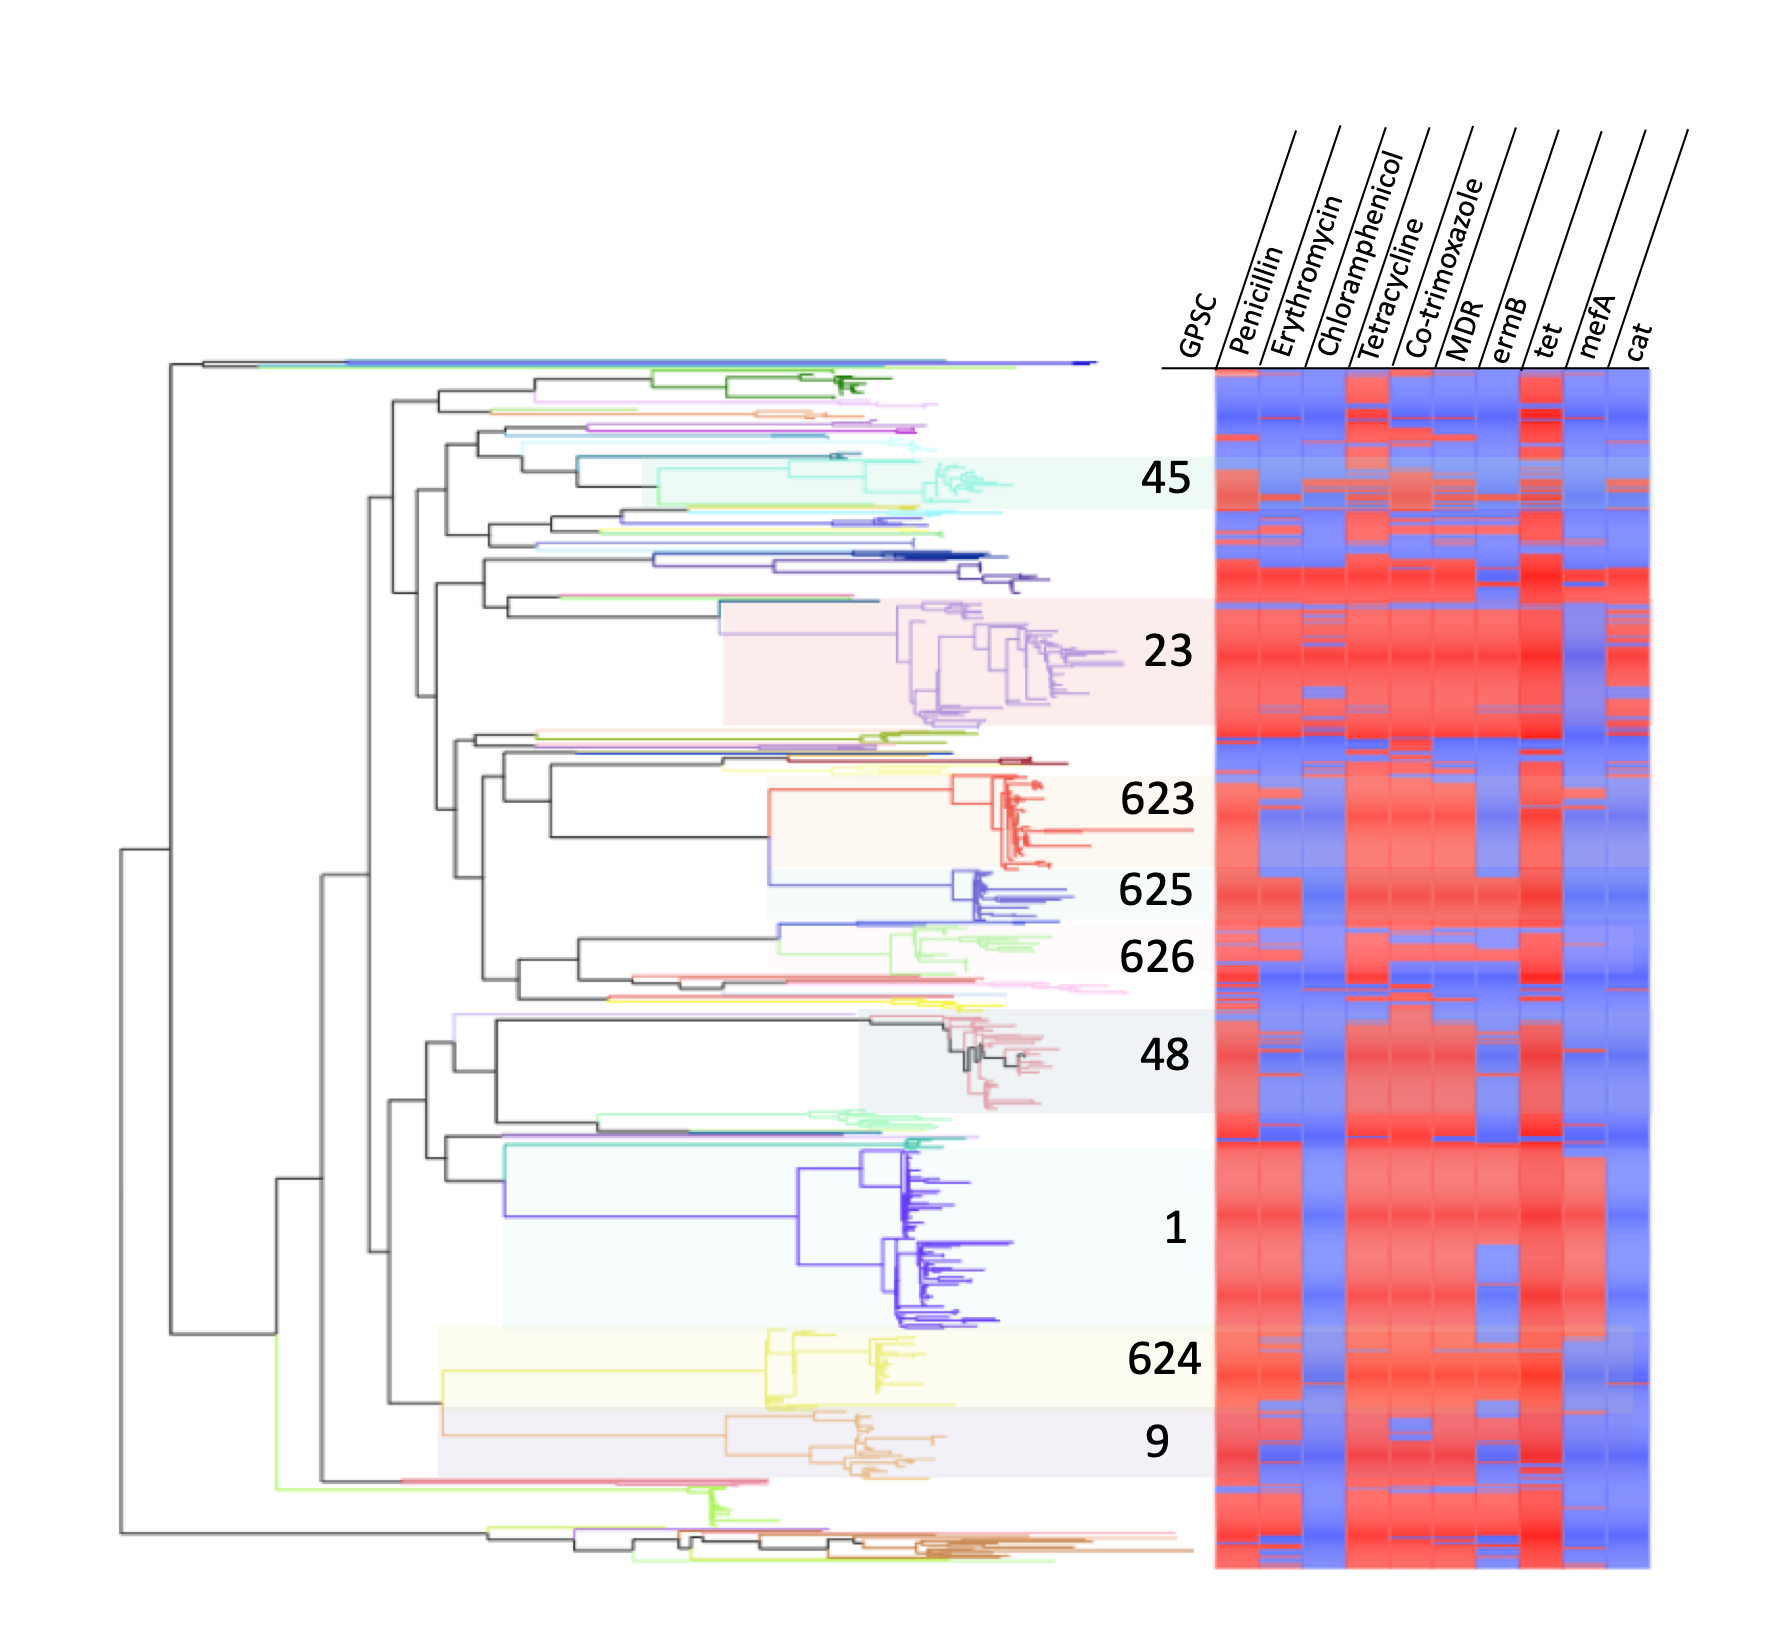
\includegraphics[width=\textwidth]{tree.png}
    \caption{Phylogenetic tree of 686 healthy carriage isolates from Cambodia. Isolated between 2013 and 2017. GPSCs at greater than 4\% prevalence in the population are highlighted. Vaccine period refers to pre- and post-PCV13 implementation in 2015.}
    \label{fig:tree}
\end{figure}
\subsection{Shifting population ecology and strain prevalence}
There was a significant increased prevalence of multiple NVTs post-vaccination including NVTs 23A (N=28, 96.3\% GPSC626; p=0.03, OR 2.86 [95\% Confidence Intervals 1.05-9.79]), 34 (N=24, 100\% GPSC45; p=0.01, OR 4.38 [1.29-23.15]), and 6D (N=9, 87.5\% GPSC16; p=0.02, OR Inf, [1.2-Inf]) \ref{tab:seroShifts} These serotype fluctuations corroborate previous findings from this region specifically the increase in NVT 34 and 23A and the decrease in VT 19F \cite{turnerImpact13ValentPneumococcal2020}. These serotypes haven't been associated with increased invasive disease potential \cite{balsellsRelativeInvasiveDisease2018}.
\\Each of the expanding NVT serotypes were on genetic backgrounds which underwent significant prevalence changes following the implementation of PCV13. For example, GPSC626 underwent a significant expansion and loss of serotype diversity following PCV13 (N=28, p=0.03, OR 2.84 [1.04-9.69]). In the pre-PCV13 population it comprised VT 23F (1, 20\%), and NVT 11A (N=1, 20\%), and 23A (3, 60\%). whereas, the post-PCV13 population GPSC626 only comprised NVT 23A (N=23, 100\%).  This rapid shift to 100\% of the sampled GPSC626 expressing serotype 23A may indicate that this serotype is more viable on this genetic background than the other NVTs present in GPSC626 pre-PCV13 (11A and 23A). A similar success story of a single serotype exists on the genetic backbone of GPSC45. Although the increasing prevalence of GPSC45 is not overall significant the predominantly increasing serotype on this backbone, serotype 34, is. Prior to PCV13 GPSC45 comprised NVT 34 (N=3, 60\%), 15B/C (N=1, 20\%) and 35F (1, 20\%), whereas following PCV13 it only comprised NVT 34 (N=21, 100\%). 
\\GPSC16, on the other hand, comprised more serotypes in the post-PCV13 population than in the pre-PCV population, and significantly increased in prevalence (N=20, p =0.04, OR 3.48 [0.99-18.7]). Prior to PCV13 GPSC16 comprised VT serotype 23F (N=2, 66.66\%) and 18C (N=1, 33.33\%); while following PCV13 implementation it comprised VTs 18C (N=8, 47.06\%) and 23F (N=1, 5.88\%); and NVTs 6D (N=7, 47.18\%) and 24 (N=1, 5.88\%).
\\The only VT with decreasing prevalence in the post-PCV13 population was 19F(N=52, 98.1\% predominant GPSC1; p=0.02, OR 0.49 [0.26-0.90]). All serotype 19F genomes were on a GPSC1 backbone (N=102, p=0.01, OR 0.54[0.35-0.85]). It is the primary genetic background for, and is mostly restricted to VT 19A and 19F, but grew to include VT 23F (N=1, 1.92\%) in the post-PCV13 population (Figure \ref{fig:prepost})(Table \ref{tab:gpscShifts})(Table \ref{tab:seroShifts}). 
\\Although a previous studies in Cambodia identified increases in NVTs 15B/C and 15A they did not significantly increase in this study \cite{turnerImpact13ValentPneumococcal2020}. This discrepancy may reflect our exclusion of disease isolate while the previously noted increase in serotype 15A was associated with disease. Of the 19 serotype 15A genomes 13 of them are on a GPSC9 genetic background (68.4\%). This is a notable strain in the region due to its possession of an IPD associated NVT serotype 15A \cite{turnerImpact13ValentPneumococcal2020}. GPSC9 is additionally notable as neighboring Thailand
\begin{figure}
    \centering
    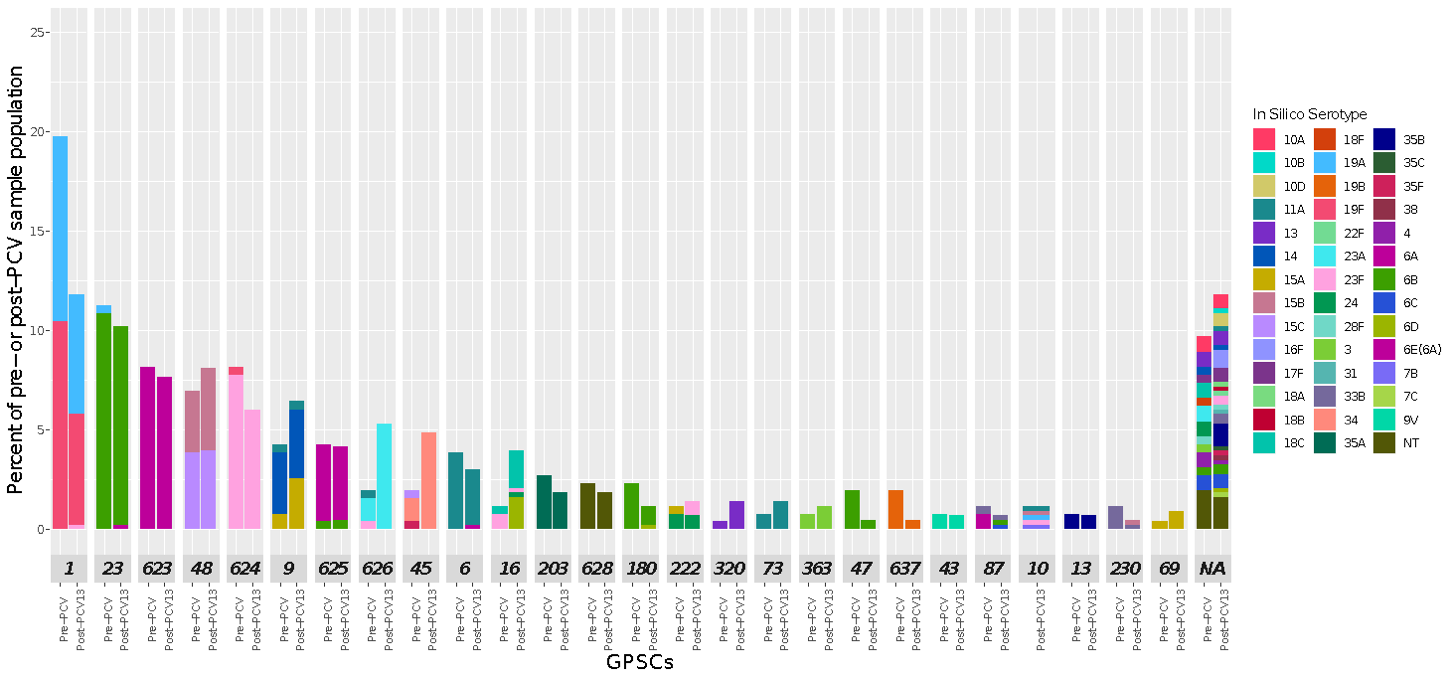
\includegraphics[width=\textwidth]{prepost_gpsc.png}
    \caption{Prevalence table of pre- and post-PCV13 GPSC isolates filled in by in silico serotype. The x axis is GPSC and vaccine period. The y axis is percent of the pre or post population. Significant prevalence changes in GPSC for 1,16, 45, and 626.  Serotype prevalence differed pre- and post- for 19F, 23A, 34, and 6D.}
    \label{fig:prepost}
\end{figure}
\subsection{Antimicrobial resistance}
\subsubsection{Phenotypic \& in-silico concordance}
Antimicrobial resistance is prevalent in this population and concordance between WGS and phenotypic antibiotic resistance for all assessed antibiotics is greater than 90\% with the discrepancies explained more frequently by false positive AMR identification in-silico than false negatives. The CDC in-silico drug resistance pipeline has not been previously validated in this region, the high concordance indicates a strong potential to use it for future genomic surveillance on S. pneumoniae. (Table \ref{tab:drug_conc}). 
\subsubsection{Prevalence}
The prevalence of predicted antimicrobial resistance is summarized in table 3. As expected, the results are concordant with previous studies from Cambodia. \cite{turnerPneumococcalInfectionChildren2015}. There is no significant changes in prevalence between the vaccine period (pre-PCV or post-PCV13)(Table \ref{tab:amr_prepost}). There is, however, a significant correlation between VTs and antimicrobial resistance exception of ermB (Table \ref{tab:VT_AMR}). Assuming PCV13 has a 100\% efficacy to eliminate VTs from the population, prevalence of antibiotic resistance in this population should decrease. This may lead to overall AMR reduction in this population as the VTs decrease. Alternatively, the genetic backgrounds containing VT and AMR may persist and expand to escape the vaccine. Additionally, concurrence of many evaluated AMR genes and antimicrobial susceptibility patterns may indicate co-selection in this population (Figure\ref{fig:tree}). 
\subsubsection{Penicillin}
There was a high prevalence of penicillin non-susceptibility, driven by \textbf{PBP??} in this population. The most prevalent GPSCs in the region (GPSC1, GPSC23, GPSC623, GPSC48, GPSC624, GPSC9, GPSC625) were all 100\% penicillin non-susceptible and comprised 70\% of the total penicillin resistance in the region\ref{fig:tree}. 
\subsubsection{Erythromycin}
The odds of GPSC1 carrying the ermB gene is higher than other strains in the region (p=0.0148, OR 1.71[1.09-2.67]). Furthermore, serotype 23F, the serotype identified in the post-PCV13 population of GPSC1, was significantly associated with erythromycin resistance (p=0.00347, OR 2.37[1.28-4.56]) and also had increased odds for ermB (p=0.00019, OR 2.85[1.58-5.24]) possibly as a result of both locis association with GPSC1. Serotypes 11A (p=0.0013, OR 3.078[1.46-6.75]), 61\% of which are on a GPSC6 genetic backbone,  and serotype 15A of which 68\% are on a GPSC9 backbone (p=0.0075,OR 3.68[1.28=11.96]) also had high risk of carrying the ermB gene\ref{fig:tree}. GPSC9 had a post-PCV13 15A expansion while GPSC6 decreased post-PCV13
\subsubsection{Chloramphenicol}
Chloramphenicol resistance was significantly associated with the successful serotype 34 (p=0.009, OR 3.43[1.23-8.81]) and correspondingly with the GPSC45 genetic background into which serotype 34 expanded (p=0.015, OR 3.04[1.10-7.64]). Furthermore, GPSC45 carries the chloramphenicol acetyltransferase gene (cat) (p=0.0.01, OR 3.08 [1.12-7.74]) at a higher prevalence than other strains in the region\ref{fig:tree}. 
\subsubsection{Tetracycline}
The tetracycline gene, tetM, was particularly prevalent in this population, and was carried in more serotypes from the pre-(N=26 serotypes) to the post-populations (N=36 serotypes). The prevalence of tetM in the post vaccine populations increased significantly in non-vaccine type serotypes 23A (N=26, GPSC626, p= 0.01, OR 4.81 [1.43-25.3]) and 6D (N = 9, GPSC16, p = 0.02, OR – Inf [1.20-inf]), and decreased significantly in vaccine type 19F (N=52, 98.1\% GPSC1; p = 0.02, OR 0.49 [0.26-0.90]). All but two serotype 6A genomes (83, 97.6\%) were tetracycline resistant (p=0.0038, OR, 9.5[1.6-386]). Of these 53 (64.6\%) were on a GPSC623 genetic background while 26 (31.7\%) were on a GPSC625 genetic background. All GPSC625 isolates carried tetM1 while all but one GPSC623 carried tetM1. Only one GPSC623, serotype 6A genome did not carry a tet gene. 
\\There was not a significant increase of tetM in the post-PCV population overall. The GPSCs with increased risk of carrying tetM included GPSC23 (97.3\% Serotype 6B, p=0.01, OR 4.94[1.27-42.5]) and GPSC48 (100\% Serotype 15B/C, p=0.02, OR 7.09[1.18-288.96]). Their predominant serotypes were also at increased risk. 
\\mefA, the macrolide efflux pump gene was associated with the expanding serotype 6D (p=0.00034, OR 14.11[2.647-140.97]) on a GPSC16 genetic background\ref{fig:tree}.
\subsubsection{Multi-drug resistance}
Multi-drug resistance (MDR) was characterized as resistance to a minimum of three different classes of antimicrobials. There was no significant difference in MDR from the pre-PCV (79\% MDR) to post-PCV13 (76\% MDR) populations however there was a higher prevalence of MDR in the VT serotypes (91\% MDR) compared with the NVT serotypes (62\% MDR). This may imply that with more time for the vaccine to block transmission chains of VT serotypes a concurrent drop in AMR may occur in this region\ref{fig:tree}. 
\subsubsection{AMR in Cambodia}
Many of the highly prevalent GPSCs in this population include high prevalence antimicrobial non-susceptible isolates. AMR may help explain the post-PCV13 expansion of some serotypes as in the case of NVT 34. Cambodia has reduced its usage of chloramphenicol in recent years so it is notable that this gene has been retained and may be a by-product of historic overuse. The tetracycline resistance gene \textit{tetM} and \textit{mefA}, are both associated with expanding NVT serotypes . Overall, however, the clear association between VT and AMR is tentatively promising for vaccine driven AMR reduction.
\section{Conclusions and Future}
It is clear that non-vaccine serotypes are being driven up by the use of PCV13 in Cambodia and the genetic background of these successful capsular types vary between expanding diversely as with GPSC16 or in the case of GPSC626 and GPSC45 expanding with a single serotype becoming predominant. GPSC16 likely included several low prevalence serotypes which were unmasked by inclusion of 23F in the vaccine, and although expansion of 18C is disconcerting 18C has a lower overall prevalence. A single serotype may subjugate the others diminishing diversity; as such serotypes 6D should be closely monitored, as should GPSC16 which has the propensity to carry a diversity of \textit{cps} loci. It does not appear that the 6A and 6B inclusion in PCV13 is cross-protective against serotype 6D indicated by its expansion. VT serotype 18C exists on the same GPSC16, genetic backbone as 6D and appears undeterred by the vaccine in the study population. Antimicrobial resistance is prevalent in this population and is associated with some expanding serotypes and strains although its association with VT serotypes may encourage overall decline (Table \ref{tab:VT_AMR}). 
\begin{table}[hbt!]
\caption{Description of sample collection period, sex, age, and vaccine status for 686 healthy Cambodian children stratified by pre-PCV (N=258) and post-PCV13(N=428) }
\label{tab:descstats}
\resizebox{\textwidth}{!}{%
\begin{tabular}{lllll}
                                &           & Pre-PCV (N=258) & Post-PCV13 (N=428) & Total (N=686)   \\
\multicolumn{2}{l}{Collection Period}       & 2013–2015       & 2016-2017          &                 \\
Female gender (\%)              & N (\%)    & 117 (45.3\%)    & 201 (47.0\%)       & 318 (46.4\%)    \\
\multirow{2}{*}{Age (months)}   & Mean (SD) & 17.779 (13.941) & 18.079 (13.736)    & 17.966 (13.804) \\
                                & Range     & 2-48            & 1-60               & 1-60            \\
\multirow{3}{*}{Vaccine Status} & NVT       & 107 (41.5\%)    & 230 (53.7\%)       & 337 (49.1\%)    \\
                                & PCV13     & 143 (55.4\%)    & 185 (43.2\%)       & 328 (47.8\%)    \\
                                & NT        & 8 (3.1\%)       & 13 (3.0\%)         & 21 (3.0\%)     
\end{tabular}%
}
\end{table}
\begin{table}[hbt!]
\caption{Concordance rates between genotypic and phenotypic antimicrobial resistance data. False positive is referred to as "major discrepancy by the US-FDA", while false negative is referred to as "very major discrepancy" by the US-FDA.}
\label{tab:drug_conc}
\resizebox{\textwidth}{!}{%
\begin{tabular}{llll}
Antibiotic Evaluated                      & Concordance & \begin{tabular}[c]{@{}l@{}}Discordant \\    \\ (False positive by WGS)\end{tabular} & \begin{tabular}[c]{@{}l@{}}Discordant \\    \\ (False negative by WGS)\end{tabular} \\
MDR                                 & 651 (94.9)  & 27 (3.9)                                                                            & 8 (1.2)                                                                             \\
Penicillin (Meningitis   threshold) & 656 (95.6)  & 23 (3.4)                                                                            & 6 (0.9)                                                                             \\
Erythromycin                        & 679 (99)    & 5 (0.7)                                                                             & 2 (0.3)                                                                             \\
Chloramphenicol                     & 682 (99.4)  & 2 (0.3)                                                                             & 2 (0.3)                                                                             \\
Tetracycline                        & 646 (94.2)  & 22 (3.2)                                                                            & 18 (2.6)                                                                            \\
Co-trimoxazole                      & 648 (94.5)  & 38 (5.5)                                                                            & -                                                                                  
\end{tabular}%
}
\end{table}
\begin{table}[hbt!]
\caption{Prevalence of antimicrobial non-susceptible isolates pre and post PCV13 in Cambodia for MDR (NS for 2 or more), penicillin (using the resistance threshold for meningitis), erythromycin, chloramphenicol, tetracycline, co-trimoxazole, and macrolides resistance: mef,ermB,cat, and tetM.}
\label{tab:amr_prepost}
\resizebox{\textwidth}{!}{%
\begin{tabular}{llll}
                                   & pre-PCV (N=258) & post-PCV13 (N=428) & Total (N=686) \\
MDR                                & 204 (79.1\%)    & 325 (75.9\%)       & 529 (77.1\%)  \\
Penicilin (Meningitis   threshold) & 210 (81.4\%)    & 355 (82.9\%)       & 565 (82.4\%)  \\
Erythromycin                       & 142 (55.0\%)    & 211 (49.3\%)       & 353 (51.5\%)  \\
Chloramphenicol                    & 30 (11.6\%)     & 61 (14.3\%)        & 91 (13.3\%)   \\
Tetracycline                       & 231 (89.5\%)    & 392 (91.6\%)       & 623 (90.8\%)  \\
Co-trimoxazole                     & 228 (88.4\%)    & 346 (80.8\%)       & 574 (83.7\%)  \\
mef presence                       & 61 (23.6\%)     & 82 (19.2\%)        & 143 (20.8\%)  \\
ermB presence                      & 107 (41.5\%)    & 155 (36.2\%)       & 262 (38.2\%)  \\
cat presence                       & 30 (11.6\%)     & 61 (14.3\%)        & 91 (13.3\%)   \\
tetM presence                      & 226 (87.6\%)    & 383 (89.5\%)       & 609 (88.8\%) 
\end{tabular}%
}
\end{table}
\begin{table}[hbt!]
\caption{Relationship between antimicrobial resistance (AMR) and VT serotypes for 5 different antimicrobials and macrolide resistance genes. Adjusting for multiple testing (threshold 0.005) all except \textit{tet} are significantly associated with VT serotypes. }
\label{tab:VT_AMR}
\resizebox{\textwidth}{!}{%
\begin{tabular}{lll}
Antibiotic      & Odds Ratio (95\% Confidence Intervals) & p-value  \\
MDR             & 6.46{[}4.09-10.5{]}                    & 6.76E-20 \\
Penicillin      & 6.39{[}3.79-11.24{]}                   & 8.44E-16 \\
Erythromycin    & 6.76{[}4.76-9.68{]}                    & 3.79E-31 \\
Tetracycline    & 2.65{[}1.46-4.98{]}                    & 5.30E-04 \\
Chloramphenicol & 3.56{[}2.12-6.17{]}                    & 1.39E-07 \\
Co-trimoxazole  & 6.55{[}3.8-11.86{]}                    & 3.86E-15 \\
ermB            & 3.55{[}2.52-5.02{]}                    & 1.28E-14 \\
mefA            & 9.11{[}5.44-15.96{]}                   & 1.28E-23 \\
cat             & 3.56{[}2.12-6.17{]}                    & 1.39E-07 \\
tet             & 2.07{[}1.23-3.56{]}                    & 0.0050  
\end{tabular}%
}
\end{table}
\begin{table}[hbt!]
\caption{Shifts in GPSC prevalence from pre-PCV to post-PCV13 ordered from increasing to decreasing overall prevalence by rows. }
\label{tab:gpscShifts}
\resizebox{\textwidth}{!}{%
\begin{tabular}{cccc}
GPSC & Pre-PCV (N=258) & Post-PCV13 (N=428) & Total (N=686) \\
1    & 51 (19.8\%)     & 51 (11.9\%)        & 102 (14.9\%)  \\
23   & 29 (11.2\%)     & 44 (10.3\%)        & 73 (10.6\%)   \\
623  & 21 (8.1\%)      & 33 (7.7\%)         & 54 (7.9\%)    \\
48   & 18 (7.0\%)      & 35 (8.2\%)         & 53 (7.7\%)    \\
624  & 21 (8.1\%)      & 26 (6.1\%)         & 47 (6.9\%)    \\
9    & 11 (4.3\%)      & 28 (6.5\%)         & 39 (5.7\%)    \\
625  & 11 (4.3\%)      & 18 (4.2\%)         & 29 (4.2\%)    \\
626  & 5 (1.9\%)       & 23 (5.4\%)         & 28 (4.1\%)    \\
45   & 5 (1.9\%)       & 21 (4.9\%)         & 26 (3.8\%)    \\
6    & 10 (3.9\%)      & 13 (3.0\%)         & 23 (3.4\%)    \\
16   & 3 (1.2\%)       & 17 (4.0\%)         & 20 (2.9\%)    \\
203  & 7 (2.7\%)       & 8 (1.9\%)          & 15 (2.2\%)    \\
628  & 6 (2.3\%)       & 8 (1.9\%)          & 14 (2.0\%)    \\
180  & 6 (2.3\%)       & 5 (1.2\%)          & 11 (1.6\%)    \\
222  & 3 (1.2\%)       & 6 (1.4\%)          & 9 (1.3\%)     \\
73   & 2 (0.8\%)       & 6 (1.4\%)          & 8 (1.2\%)     \\
47   & 5 (1.9\%)       & 2 (0.5\%)          & 7 (1.0\%)     \\
320  & 1 (0.4\%)       & 6 (1.4\%)          & 7 (1.0\%)     \\
363  & 2 (0.8\%)       & 5 (1.2\%)          & 7 (1.0\%)     \\
637  & 5 (1.9\%)       & 2 (0.5\%)          & 7 (1.0\%)     \\
87   & 3 (1.2\%)       & 3 (0.7\%)          & 6 (0.9\%)     \\
10   & 0 (0.0\%)       & 5 (1.2\%)          & 5 (0.7\%)     \\
13   & 2 (0.8\%)       & 3 (0.7\%)          & 5 (0.7\%)     \\
43   & 2 (0.8\%)       & 3 (0.7\%)          & 5 (0.7\%)     \\
69   & 1 (0.4\%)       & 4 (0.9\%)          & 5 (0.7\%)     \\
230  & 3 (1.2\%)       & 2 (0.5\%)          & 5 (0.7\%)     \\
122  & 1 (0.4\%)       & 3 (0.7\%)          & 4 (0.6\%)     \\
134  & 2 (0.8\%)       & 2 (0.5\%)          & 4 (0.6\%)     \\
158  & 0 (0.0\%)       & 4 (0.9\%)          & 4 (0.6\%)     \\
653  & 1 (0.4\%)       & 3 (0.7\%)          & 4 (0.6\%)     \\
40   & 1 (0.4\%)       & 2 (0.5\%)          & 3 (0.4\%)     \\
59   & 0 (0.0\%)       & 3 (0.7\%)          & 3 (0.4\%)     \\
142  & 2 (0.8\%)       & 1 (0.2\%)          & 3 (0.4\%)     \\
147  & 0 (0.0\%)       & 3 (0.7\%)          & 3 (0.4\%)     \\
162  & 2 (0.8\%)       & 1 (0.2\%)          & 3 (0.4\%)     \\
319  & 0 (0.0\%)       & 3 (0.7\%)          & 3 (0.4\%)     \\
654  & 0 (0.0\%)       & 3 (0.7\%)          & 3 (0.4\%)     \\
671  & 2 (0.8\%)       & 1 (0.2\%)          & 3 (0.4\%)     \\
28   & 1 (0.4\%)       & 1 (0.2\%)          & 2 (0.3\%)     \\
60   & 1 (0.4\%)       & 1 (0.2\%)          & 2 (0.3\%)     \\
106  & 2 (0.8\%)       & 0 (0.0\%)          & 2 (0.3\%)     \\
383  & 1 (0.4\%)       & 1 (0.2\%)          & 2 (0.3\%)     \\
5    & 1 (0.4\%)       & 0 (0.0\%)          & 1 (0.1\%)     \\
14   & 0 (0.0\%)       & 1 (0.2\%)          & 1 (0.1\%)     \\
18   & 0 (0.0\%)       & 1 (0.2\%)          & 1 (0.1\%)     \\
20   & 0 (0.0\%)       & 1 (0.2\%)          & 1 (0.1\%)     \\
22   & 0 (0.0\%)       & 1 (0.2\%)          & 1 (0.1\%)     \\
30   & 1 (0.4\%)       & 0 (0.0\%)          & 1 (0.1\%)     \\
37   & 1 (0.4\%)       & 0 (0.0\%)          & 1 (0.1\%)     \\
38   & 0 (0.0\%)       & 1 (0.2\%)          & 1 (0.1\%)     \\
51   & 1 (0.4\%)       & 0 (0.0\%)          & 1 (0.1\%)     \\
57   & 0 (0.0\%)       & 1 (0.2\%)          & 1 (0.1\%)     \\
95   & 0 (0.0\%)       & 1 (0.2\%)          & 1 (0.1\%)     \\
215  & 0 (0.0\%)       & 1 (0.2\%)          & 1 (0.1\%)     \\
240  & 0 (0.0\%)       & 1 (0.2\%)          & 1 (0.1\%)     \\
397  & 1 (0.4\%)       & 0 (0.0\%)          & 1 (0.1\%)     \\
400  & 0 (0.0\%)       & 1 (0.2\%)          & 1 (0.1\%)     \\
495  & 0 (0.0\%)       & 1 (0.2\%)          & 1 (0.1\%)     \\
519  & 0 (0.0\%)       & 1 (0.2\%)          & 1 (0.1\%)     \\
794  & 1 (0.4\%)       & 0 (0.0\%)          & 1 (0.1\%)     \\
795  & 1 (0.4\%)       & 0 (0.0\%)          & 1 (0.1\%)     \\
797  & 0 (0.0\%)       & 1 (0.2\%)          & 1 (0.1\%)     \\
799  & 0 (0.0\%)       & 1 (0.2\%)          & 1 (0.1\%)     \\
800  & 1 (0.4\%)       & 0 (0.0\%)          & 1 (0.1\%)     \\
801  & 0 (0.0\%)       & 1 (0.2\%)          & 1 (0.1\%)     \\
802  & 0 (0.0\%)       & 1 (0.2\%)          & 1 (0.1\%)     \\
804  & 0 (0.0\%)       & 1 (0.2\%)          & 1 (0.1\%)     \\
805  & 0 (0.0\%)       & 1 (0.2\%)          & 1 (0.1\%)     \\
806  & 0 (0.0\%)       & 1 (0.2\%)          & 1 (0.1\%)     \\
819  & 1 (0.4\%)       & 0 (0.0\%)          & 1 (0.1\%)    
\end{tabular}%
}
\end{table}

\begin{table}[hbt!]
\caption{Shifts in serotype from pre-PCV to post-PCV13 ordered from increasing to decreasing overall prevalence by rows. }
\label{tab:seroShifts}
\resizebox{\textwidth}{!}{%
\begin{tabular}{cccc}
\multicolumn{1}{l}{In Silico   Serotypes} & Pre-PCV (N=258) & Post-PCV13 (N=428) & Total (N = 686) \\
6B                                        & 41 (15.9\%)     & 54 (12.6\%)        & 95 (13.8\%)     \\
6A                                        & 33 (12.8\%)     & 50 (11.7\%)        & 83 (12.1\%)     \\
23F                                       & 23 (8.9\%)      & 34 (7.9\%)         & 57 (8.3\%)      \\
19A                                       & 25 (9.7\%)      & 27 (6.3\%)         & 52 (7.6\%)      \\
19F                                       & 28 (10.9\%)     & 24 (5.6\%)         & 52 (7.6\%)      \\
11A                                       & 14 (5.4\%)      & 22 (5.1\%)         & 36 (5.2\%)      \\
15B                                       & 8 (3.1\%)       & 20 (4.7\%)         & 28 (4.1\%)      \\
15C                                       & 11 (4.3\%)      & 17 (4.0\%)         & 28 (4.1\%)      \\
23A                                       & 5 (1.9\%)       & 23 (5.4\%)         & 28 (4.1\%)      \\
NT                                        & 11 (4.3\%)      & 15 (3.5\%)         & 26 (3.8\%)      \\
14                                        & 9 (3.5\%)       & 16 (3.7\%)         & 25 (3.6\%)      \\
34                                        & 3 (1.2\%)       & 21 (4.9\%)         & 24 (3.5\%)      \\
15A                                       & 4 (1.6\%)       & 15 (3.5\%)         & 19 (2.8\%)      \\
35A                                       & 7 (2.7\%)       & 8 (1.9\%)          & 15 (2.2\%)      \\
13                                        & 3 (1.2\%)       & 9 (2.1\%)          & 12 (1.7\%)      \\
18C                                       & 3 (1.2\%)       & 8 (1.9\%)          & 11 (1.6\%)      \\
35B                                       & 2 (0.8\%)       & 8 (1.9\%)          & 10 (1.5\%)      \\
6D                                        & 0 (0.0\%)       & 9 (2.1\%)          & 9 (1.3\%)       \\
24                                        & 4 (1.6\%)       & 4 (0.9\%)          & 8 (1.2\%)       \\
3                                         & 3 (1.2\%)       & 5 (1.2\%)          & 8 (1.2\%)       \\
33B                                       & 4 (1.6\%)       & 4 (0.9\%)          & 8 (1.2\%)       \\
19B                                       & 5 (1.9\%)       & 2 (0.5\%)          & 7 (1.0\%)       \\
6C                                        & 2 (0.8\%)       & 4 (0.9\%)          & 6 (0.9\%)       \\
10A                                       & 2 (0.8\%)       & 3 (0.7\%)          & 5 (0.7\%)       \\
9V                                        & 2 (0.8\%)       & 3 (0.7\%)          & 5 (0.7\%)       \\
16F                                       & 0 (0.0\%)       & 4 (0.9\%)          & 4 (0.6\%)       \\
17F                                       & 1 (0.4\%)       & 3 (0.7\%)          & 4 (0.6\%)       \\
10D                                       & 0 (0.0\%)       & 3 (0.7\%)          & 3 (0.4\%)       \\
4                                         & 2 (0.8\%)       & 1 (0.2\%)          & 3 (0.4\%)       \\
28F                                       & 1 (0.4\%)       & 1 (0.2\%)          & 2 (0.3\%)       \\
35F                                       & 1 (0.4\%)       & 1 (0.2\%)          & 2 (0.3\%)       \\
10B                                       & 0 (0.0\%)       & 1 (0.2\%)          & 1 (0.1\%)       \\
18A                                       & 0 (0.0\%)       & 1 (0.2\%)          & 1 (0.1\%)       \\
18B                                       & 0 (0.0\%)       & 1 (0.2\%)          & 1 (0.1\%)       \\
18F                                       & 1 (0.4\%)       & 0 (0.0\%)          & 1 (0.1\%)       \\
22F                                       & 0 (0.0\%)       & 1 (0.2\%)          & 1 (0.1\%)       \\
31                                        & 0 (0.0\%)       & 1 (0.2\%)          & 1 (0.1\%)       \\
35C                                       & 0 (0.0\%)       & 1 (0.2\%)          & 1 (0.1\%)       \\
38                                        & 0 (0.0\%)       & 1 (0.2\%)          & 1 (0.1\%)       \\
6E(6A)                                    & 0 (0.0\%)       & 1 (0.2\%)          & 1 (0.1\%)       \\
7B                                        & 0 (0.0\%)       & 1 (0.2\%)          & 1 (0.1\%)       \\
7C                                        & 0 (0.0\%)       & 1 (0.2\%)          & 1 (0.1\%)       \\
1                                         & 0 (0.0\%)       & 0 (0.0\%)          & 0 (0.0\%)       \\
12F                                       & 0 (0.0\%)       & 0 (0.0\%)          & 0 (0.0\%)       \\
21                                        & 0 (0.0\%)       & 0 (0.0\%)          & 0 (0.0\%)       \\
20                                        & 0 (0.0\%)       & 1 (0.2\%)          & 1 (0.1\%)       \\
22                                        & 0 (0.0\%)       & 1 (0.2\%)          & 1 (0.1\%)       \\
30                                        & 1 (0.4\%)       & 0 (0.0\%)          & 1 (0.1\%)       \\
37                                        & 1 (0.4\%)       & 0 (0.0\%)          & 1 (0.1\%)       \\
38                                        & 0 (0.0\%)       & 1 (0.2\%)          & 1 (0.1\%)       \\
51                                        & 1 (0.4\%)       & 0 (0.0\%)          & 1 (0.1\%)       \\
57                                        & 0 (0.0\%)       & 1 (0.2\%)          & 1 (0.1\%)       \\
95                                        & 0 (0.0\%)       & 1 (0.2\%)          & 1 (0.1\%)       \\
215                                       & 0 (0.0\%)       & 1 (0.2\%)          & 1 (0.1\%)       \\
240                                       & 0 (0.0\%)       & 1 (0.2\%)          & 1 (0.1\%)       \\
397                                       & 1 (0.4\%)       & 0 (0.0\%)          & 1 (0.1\%)       \\
400                                       & 0 (0.0\%)       & 1 (0.2\%)          & 1 (0.1\%)       \\
495                                       & 0 (0.0\%)       & 1 (0.2\%)          & 1 (0.1\%)       \\
519                                       & 0 (0.0\%)       & 1 (0.2\%)          & 1 (0.1\%)       \\
794                                       & 1 (0.4\%)       & 0 (0.0\%)          & 1 (0.1\%)       \\
795                                       & 1 (0.4\%)       & 0 (0.0\%)          & 1 (0.1\%)       \\
797                                       & 0 (0.0\%)       & 1 (0.2\%)          & 1 (0.1\%)       \\
799                                       & 0 (0.0\%)       & 1 (0.2\%)          & 1 (0.1\%)       \\
800                                       & 1 (0.4\%)       & 0 (0.0\%)          & 1 (0.1\%)       \\
801                                       & 0 (0.0\%)       & 1 (0.2\%)          & 1 (0.1\%)       \\
802                                       & 0 (0.0\%)       & 1 (0.2\%)          & 1 (0.1\%)       \\
804                                       & 0 (0.0\%)       & 1 (0.2\%)          & 1 (0.1\%)       \\
805                                       & 0 (0.0\%)       & 1 (0.2\%)          & 1 (0.1\%)       \\
806                                       & 0 (0.0\%)       & 1 (0.2\%)          & 1 (0.1\%)       \\
819                                       & 1 (0.4\%)       & 0 (0.0\%)          & 1 (0.1\%)      
\end{tabular}%
}
\end{table}
\newpage
\FloatBarrier
\printbibliography
\end{document}